\documentclass[a4paper, 11pt]{article}

\usepackage{geometry}
\usepackage{setspace}
\usepackage{amsmath}
\usepackage{graphicx}
\usepackage{wrapfig}
\usepackage{caption}

\geometry{left=2.5cm, right=2.5cm, top=2.5cm, bottom=2.5cm}
\graphicspath{ {./images/} }
\newcommand{\ode}{{\fontfamily{pcr}\selectfont ode45()}}
\newcommand{\dydt}{\frac{dy}{dt}}
\newcommand{\overm}[1]{\frac{#1}{m}}
\newcommand{\f}{$F_{0}$}
\newcommand{\w}{$\omega_{0}$}
\newcommand{\m}{$\mu$}

\begin{document}
	
	\begin{figure}[t]
		
\includegraphics[scale=0.25]{Logo_UA}
	\end{figure}
	
	\title{Trabalho 1 - Oscilador não-linear \\ 
		   \Large Física Computacional}
	\author{João Inácio, 93039, PL7}
	\date{06/05/2020}
	\maketitle
	
	\section{Introdução}
	
	\paragraph{}
	Este trabalho tem como principal objetivo estudar o comportamento de um oscilador não-linear. Para tal é-nos dada uma equação de movimento para um pendulo caótico e, com recurso a métodos numéricos, temos de resolver a equação diferencial não-linear. Foram usados dois métodos Runge-Kutta, a rotina \ode do MatLab, ou seja, método RK de passo adaptativo, e o método Runge-Kutta de 4ª ordem. Como a rotina \ode é de passo adaptativo podemos esperar resultados mais precisos, comparativamente ao método RK4.\\
	Um objetivo secundário deste trabalho é comparar os métodos de Runge-Kutta de 4ª ordem com a rotina \ode e com o método mais simples de resolução de ODE's, o método de Euler.
	\section{Métodos}
	\paragraph{}
	Como já mencionado na introdução, temos de resolver uma equação diferencial que representa o movimento de um pêndulo não-linear. A equação a resolver é
	\begin{equation}
		m\frac{d^2y}{dt^2}+K(y+\alpha y^3)=\mu \left[ \cos \left( \dydt \right) \right]\dydt+F_{0}cos(\omega_{0}t)
	\end{equation}
	Como a equação é do segundo grau, para aplicar os métodos numéricos temos dividi-la em duas equações de primeira ordem. Como $\dydt = v$ e $\frac{dv}{dt}=f(y,t)$, podemos substituir na equação (1). Assim, esta fica
	\begin{equation}
		\dydt = v 
	\end{equation}
	\begin{equation}
		\frac{dv}{dt} =  \overm{\mu} \left[ \cos \left( \dydt \right) \right]\dydt-\overm{K}(y+\alpha y^3)+\overm{F_{0}}cos(\omega_{0}t)
	\end{equation}
	
	\subsection{Rotina \ode}
	\paragraph{}
	A rotina \ode é uma função do MatLab, que utiliza métodos de Runge-Kutta para resolver equações diferencias ordinárias com um passo, $dt$, adaptativo. Este método, como muitos outros para resolver EDO's, apenas precisa das condições de $t_{n-1}$ para calcular as condições de $t_{n}$.
	\paragraph{}
	Esta função usa o método RK de 4ª ordem ou, no caso de ser necessário uma precisão mais elevada na estimação numérica, utiliza um RK de 5ª ordem.
	\paragraph{}
	Para utilizar este método no problema em questão temos de num ficheiro de função colocar as derivadas de primeiro grau, equações (2) e (3). Também temos de especificar o erro máximo que o método pode chegar para ter uma maior precisão. Neste caso foi utilizado um erro da ordem de $10^{-13}$.
	\paragraph{}
	Assim este método consegue uma aproximação numérica muito exata, já que adapta o passo a cada iteração e utiliza um método RK de ordem superior quando o erro é maior do que o erro mínimo especificado.
	
	\subsection{Runge-Kutta 4}
	\paragraph{}
	O método Runge-Kutta de 4ª ordem é um método numérico usado para resolver EDO's ou sistemas das mesmas, para problemas de valores iniciais.
	\paragraph{}
	Sendo a função 
	\begin{equation*}
		\dydt = f(x, t)
	\end{equation*}
	a equação diferencial a resolver, o método de RK estima a função no ponto $y_{i+1}$ através de uma média ponderada de quatro valores ou estimativas de $f(x, t)$ em pontos diferentes pertencendo ao intervalo $\left[t_{i}, t_{i+1}\right]$.
	Os diferentes pesos de cada um dos valores da média é ditado por uma tabela de \textit{Butcher}.
	\[
	\renewcommand\arraystretch{1.2}
	\begin{array}
	{c|cccc}
	0\\
	\frac{1}{2} & \frac{1}{2}\\
	\frac{1}{2} &0 &\frac{1}{2} \\
	1& 0& 0& 1\\
	\hline
	& \frac{1}{6} &\frac{1}{3} &\frac{1}{3} &\frac{1}{6} 
	\end{array}
	\]
	Esta é a tabela usada neste trabalho e, assim, com esta podemos calcular os quatro valores de $f(x, t)$ e a expressão final para o calculo de $y_{i+1}$. Para a equação (3) as quatro estimativas no intervalo $\left[t_{i}, t_{i+1}\right]$ podem ser calculadas por
	\begin{gather*}
		r_{1,y}=f_{v}\left(v_{i}\right)\\
		r_{2,y}=f_{v}\left(v_{i}+r_{1,v}\frac{dt}{2}\right)\\
		r_{3,y}=f_{v}\left(v_{i}+r_{2,v}\frac{dt}{2}\right)\\
		r_{4,y}=f_{v}\left(v_{i}+r_{3,v}dt\right)
	\end{gather*}
	O calculo de $r_{n,v}$(n=1,2,3,...,ordem do RK) é feito de maneira idêntica, apenas temos de ter em conta o incremento de $t_{i}$, que os coeficientes são a coluna mais a esquerda da tabela de \textit{Butcher}. Assim podemos encontrar as equações de $v_{i+1}$ e $v_{i+1}$
	\begin{gather}
		y_{i+1}=y_{i}+\frac{dt}{6}\left(r_{1,y}+2r_{2,y}+2r_{3,y}+r_{4,y}\right)\\
		v_{i+1}=y_{i}+\frac{dt}{6}\left(r_{1,v}+2r_{2,v}+2r_{3,v}+r_{4,v}\right)
	\end{gather}
	{\footnotesize Nota: $dt$ é o passo do método. Para uma precisão maior podemos diminuir este, ao custo de poder computacional, já que no método RK4 o erro é $\mathcal{O}(dt^{4})$, muito próximo de uma aproximação por série de Taylor.}
	
	\subsection{Método de Euler}
	\paragraph{}
	Este método é um dos métodos mais conhecidos para resolver EDO's, devido à sua simplicidade. Este método numérico faz uma aproximação da derivada de primeira ordem por a definição de derivada. Ou seja, 
	\begin{equation}
		\lim_{dt\to0}{\frac{y(x, t+dt)-y(x, t)}{dt}}=\dydt=f(x, t)
	\end{equation}
	Isto pode ser aproximado rearranjando os termos e obtemos
	\begin{equation}
		y_{n+1}=y_{n}+f(x_{n}, t_{n})dt
	\end{equation}
	\paragraph{}
	Este método é muito instável e energético, ou seja, para um $t_{final}$ muito grande o sistema começa a ganhar energia. Também é muito impreciso, com erro local $\mathcal{O}(dt)$ e um erro global $\mathcal{O}(dt^{2})$.
	O método de Euler-Cromer é um método que resolve uma derivada de segunda ordem e é idêntico a este. A única diferença é no cálculo da posição, que em vez de usar $v_{i}$, usa-se $v_{i+1}$ para melhor conservação de energia.
	
	\section{Resultados e Discussão}
	\paragraph{}
	Nesta secção vão ser apresentados os resultados. Todos os resultados foram obtidos através dos {\itshape scripts} em anexo com este relatório.
	
	\paragraph{}
	Em primeiro lugar, usando a rotina \ode do MatLab, calculamos a trajétoria e a velocidade do oscilador ao longo do intervalo de tempo $t\in [0, 150]$, este intervalo é o mesmo para todos os cálculos que se seguem.
	Nesta primeira parte fizemos variar \f e \w. Começamos com \f$=0$, ou seja, no caso em que não há oscilações forçadas, e seguidamente com \f$=0.8$ para \w$=1$ e \w$=2$.\\
	\begin{figure}[h]
		\centering
		\captionsetup{labelformat=empty}
		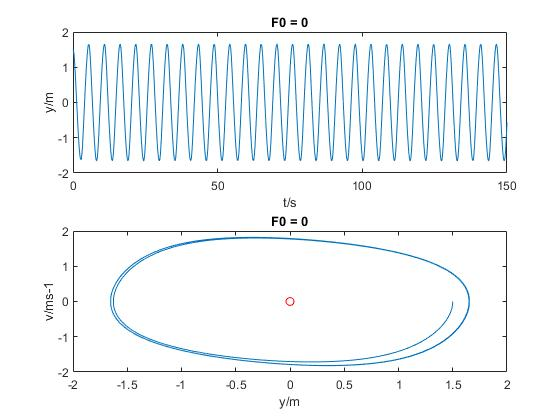
\includegraphics[width=0.5\textwidth, height=0.3\textwidth]{f0_0_phase}
		\caption{\scriptsize Gráfico 1: \f$=0$. O ponto vermelho no gráfico de baixo indica o centro, $(0, 0)$ do ciclo limite.}
	\end{figure}
	\paragraph{}
	Para \f$=0$(gráfico 1), temos, como seria de esperar, oscilações periódicas, já que a equação diferencial que descreve esta oscilação é autónoma. Também podemos verificar isto a partir do diagrama de fases (gráfico de baixo), que para uma EDO autónoma vai ter um atrator, com centro em $(0, 0)$, logo o sistema não perde energia, pois a velocidade não diminui com posição ao longo do tempo.
	\\ \\ \\ \\
	\begin{figure}[h]
		\centering
		\captionsetup{labelformat=empty}
		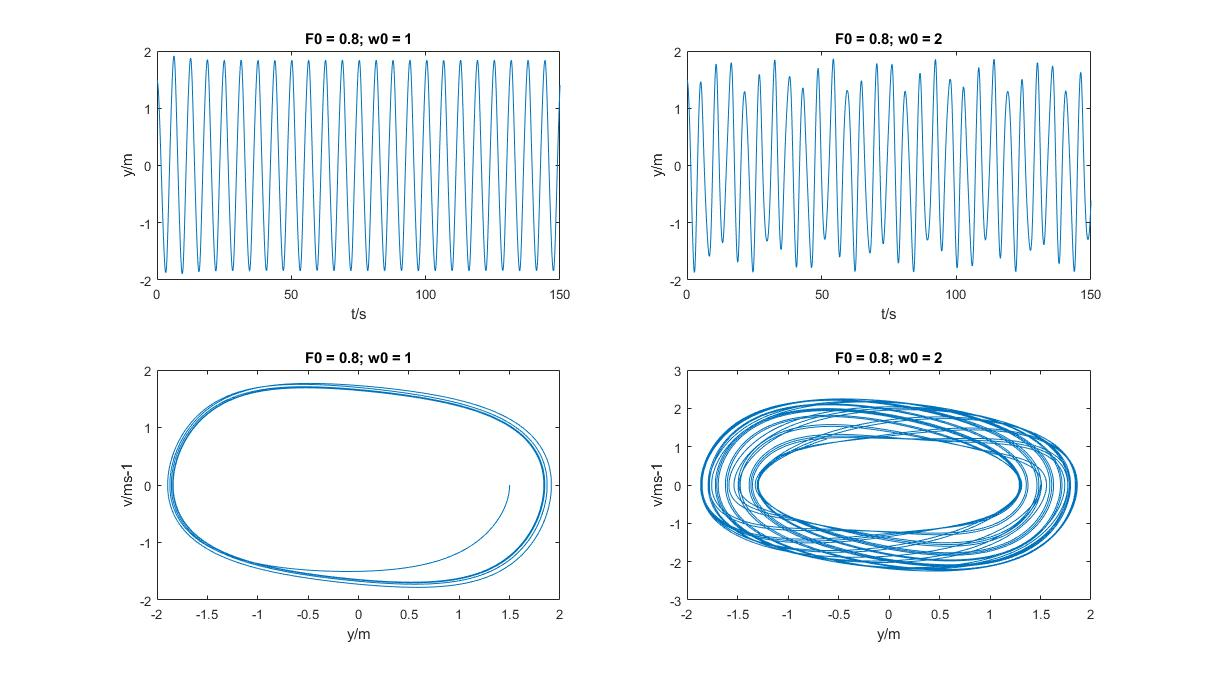
\includegraphics[width=\textwidth, height=0.4\textwidth]{f0_08_phase}
		\caption{\scriptsize Gráfico 2: \f$=0.8$, com \w$=1$(esquerda) e \w$=2$(direita).}
	\end{figure}
	\paragraph{}
	No caso de \f$=0.8$(gráfico 2), temos dois resultados diferentes para cada um dos valores de \w. Neste caso, a EDO, como já depende de $t$, é não autónoma, assim é muito mais suscetível a pequenas mudanças nas condições iniciais e nas constantes da expressão. \\
	Quando \w$=1$ (gráfico 2, esquerda), o oscilador é periódico e tem um atrator com mais voltas em relação ao primeiro caso, com \f$=0$. Assim, podemos dizer que o período da oscilação neste caso é maior do que o período do primeiro caso. Este atrator também tem um centro em $(0, 0)$. \\
	Quando \w$=2$ (gráfico 2, direita), o oscilador também é periódico como no caso de \w$=1$, e também tem um ciclo limite, contudo com consideravelmente mais voltas do que no caso de \w$=1$. Logo, o período deste é maior do que no caso anterior e ainda maior do que o do caso em que \f$=0$. \\
	Assim, em oscilações forçadas, \f$\ne0$, a frequência de oscilação esta ligada ao à frequência das oscilações forçadas. Contudo esta ligação não é proporcional a \w, uma vez que o número de voltas em \w$=2$ teria de ser o dobro das voltas em \w$=1$, o que não se verifica, pois a partir do gráfico podemos observar que é muito mais do que o dobro. 
	\begin{figure}[h]
		\centering
		\captionsetup{labelformat=empty}
		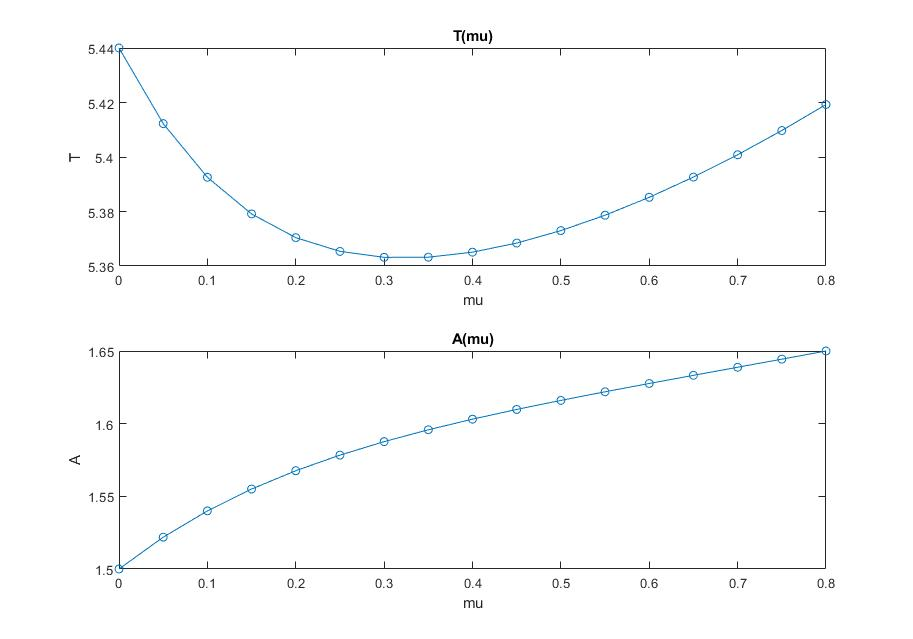
\includegraphics[width=\textwidth, height=0.55\textwidth]{A_T_mu}
		\caption{\scriptsize Gráfico 3: Período(cima) e amplitude(baixo) das oscilações em função de $\mu$, com \f$=0$}
	\end{figure}
	\paragraph{}
	Em segundo lugar, com \f$=0$, fizemos variar $\mu$, um coeficiente de amortecimento, já que é o coeficiente da primeira derivada da posição em relação ao tempo, de $0$ a $0.8$ em passos de $0.05$ para termos $17$ valores para ter uma boa amostra para fazer um gráfico(gráfico 3).
	
	\paragraph{}
	Para encontrar os períodos e amplitudes, tivemos de usar a função {\fontfamily{pcr}\selectfont lagr.m}. Esta função toma como argumentos 3 pontos, um ponto antes do máximo da função discreta, o ponto do máximo e um a seguir, para ambos os valores de {\fontfamily{pcr}\selectfont t} e {\fontfamily{pcr}\selectfont y}. Com estes valores a função encontra os valores máximos e mínimos da função  contínua. \\
	Com os todos os valores de {\fontfamily{pcr}\selectfont tMax} e {\fontfamily{pcr}\selectfont yMax} para cada valor de \m, calculamos os valores de {\fontfamily{pcr}\selectfont T} e {\fontfamily{pcr}\selectfont A} para cada valor de \m. O resultado disto é o gráfico 3.

	\paragraph{}
	Quando fazemos variar \m, o período de oscilação diminui até \m$=0.3$, a partir deste valor $T$ aumenta, e para valores do coeficiente de amortecimento maiores que $0.8$ tem uma tendência de crescimento. No caso da amplitude, podemos verificar que há um crescimento logarítmico, mesmo para \m$>0.8$.
	
	\paragraph{}
	Por fim, tivemos de fazer uma comparação entre os dois métodos descritos na secção 2. O gráfico seguinte contem os gráficos de posição em função do tempo e o gráfico de fases dos dois métodos.
	\\
	\begin{figure}[h]
		\centering
		\captionsetup{labelformat=empty}
		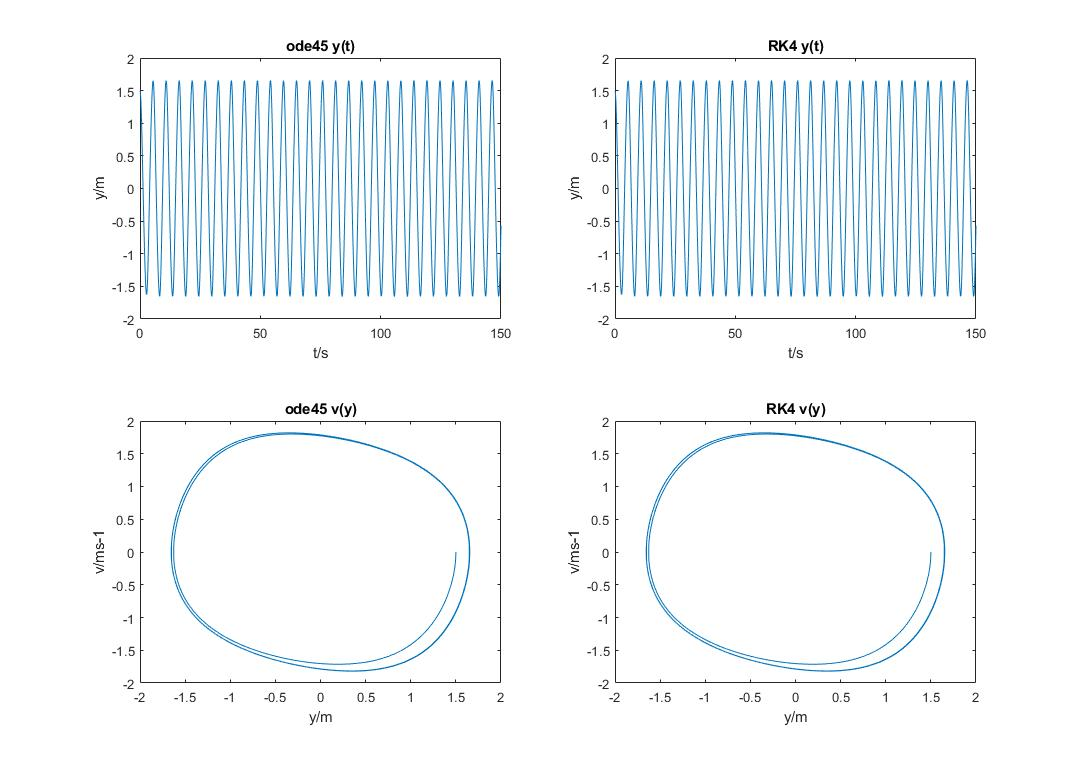
\includegraphics[width=\textwidth, height=0.5\textwidth]{ode_rk4}
		\caption{\scriptsize Gráfico 4: Comparação entre os métodos \ode e Runge-Kutta 4ª Ordem}
	\end{figure}
	\\
	\paragraph{}
	Como podemos ver pela comparação dos gráficos, para a equação de oscilação não forçada, ambos os métodos têm resultados simulares. Em ambos os gráfios $y(t)$ são iguais e o diagrama de fases também seguem a mesma forma em ambos os métodos. Se compararmos o erro de ambos os métodos ($erro=\left|y_{ode}-y_{rk4}\right|$) numa escala logarítmica, gráfico 5, podemos observar que no pior dos casos, o erro tem a ordem $1$. Esta discrepância dá-se devido ao método \ode ser ter um erro de $10^{-13}$ e ter um passo, $dt$, adaptativo, enquanto o método RK4 ter um passo fixo, $dt=0.001$, e ter um erro máximo $\mathcal{O}(dt^{4})$. Para obter um resultado mais conciso entre os dois métodos tínhamos de por um passo extremamente pequeno na execução do RK4.
	\begin{figure}[h]
		\centering
		\captionsetup{labelformat=empty}
		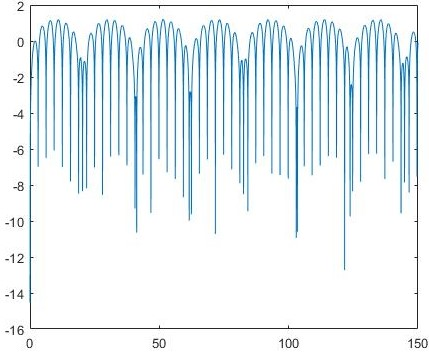
\includegraphics[scale=0.6]{erro2}
		\caption{\scriptsize Gráfico 5: Erro entre os dois métodos numa escala logarítmica.}
	\end{figure}
	\section{Conclusão}
	\paragraph{}
	Comparando os resultados obtidos na comparação do método RK4 com \ode, podemos concluir que a \ode é uma escolha mais segura, já que é mais simples de implementar no código, pois é uma função própria do MatLab, e é mais precisa, uma vez que usa um passo adaptativo ao erro máximo especificado.
	\paragraph{}
	Entre a rotina \ode e o método de Euler-Cromer, apesar de nenhum dos dois ser mais complicado de implementar, o método \ode oferece mais escolhas em relação ao erro, ja que podemos ter um erro de $10^{-13}$ e não dispender de complexidade computacional, enquanto para o método de Euler-Cromer para ter um erro parecido à \ode temos de ter um $dt$ da ordem de $-7$, pois o erro global do Euler-Cromer é $\mathcal{O}(dt^{2})$.
	\paragraph{}
	Em suma, conseguimos verificar que a \ode é mais precisa do que o método RK4, como foi previsto na introdução e também conseguimos estudar o comportamento do oscilador não-linear usando dois métodos para resolver a sua equação de movimento, o método Runge-Kutta de 4ª ordem e a rotina \ode do MatLab.
	
	
	
	
	
		
\end{document}